\newcommand\Z{\ensuremath{\mathbb{Z}}}

\section{Introduction}

Homotopy type theory~\citep{awodeywarren09identity,voevodsky11wollic} is an extension of Martin-L\"of's
intensional type
theory~\citep{nps90mltt,martinlof71itt}
 with new principles such as Voevodsky's
univalence axiom
and higher-dimensional inductive
types~\citep{lumsdaine+13hits}.  These extensions are interesting both from a
computer science perspective, where they imbue the equality apparatus of
type theory with new computational meaning, and from a mathematical
perspective, where they allow higher-dimensional mathematics to be
expressed cleanly and elegantly in type theory.  One example of
higher-dimensional mathematics is the subject of homotopy theory, a
branch of algebraic topology.  In homotopy theory, one studies
topological spaces by way of their points, paths (between points),
homotopies
(paths between paths), homotopies between
homotopies (paths between paths between paths), and so on.  This infinite tower of concepts---spaces,
points, paths, homotopies, and so on---is modeled in type theory by
types, elements of types, proofs of equality of elements, proofs of
equality of proofs of equality, and so on.  A space corresponds to a
type $A$. Points of a space correspond to elements $a,b : A$. Paths in a
space are modeled by elements of the identity type (propositional equality), which we
notate $p : a =_A b$.  Homotopies between paths $p$ and $q$ correspond
to elements of the iterated identity type $p =_{a =_A b} q$.  The
rules for the propositional equality type allow one to define the
operations on paths that are considered in homotopy theory.  These include identity paths
$\dsd{id} : a = a$ (reflexivity of equality), inverse paths $\inv p : b
= a$ when $p : a = b$ (symmetry of equality), and composition of paths
$q \comp p : a = c$ when $p : a = b$ and $q : b = c$ (transitivity of
equality), as well as homotopies relating these operations (for example,
$\dsd{id} \comp p = p$), and homotopies relating these homotopies, etc.  This
equips each type with the structure of a (weak)
\emph{$\infty$-groupoid}, as studied in higher category
theory~\citep{lumsdaine09omega,vandenberggarner10groupoids}.  In category theoretic terminology, the elements of
a type correspond to objects (or 0-cells), the proofs of equality of
elements to morphisms (1-cells), the proofs of equality of proofs of
equality to 2-morphisms (2-cells), and so on.

One basic question in algebraic topology is calculating the
\emph{homotopy groups} of a space.  Given a space $X$ with a
distinguished point $x_0$, the \emph{fundamental group of $X$ at the
  point $x_0$} (denoted $\pi_1(X,x_0)$) is the group of loops at $x_0$
up to homotopy, with composition as the group operation.  This
fundamental group is the first in a sequence of \emph{homotopy groups},
which provide higher-dimensional information about a space: the homotopy
groups $\pi_n(X,x_0)$ ``count'' the $n$-dimensional loops in that space
up to homotopy.  $\pi_2(X,x_0)$ is the group of homotopies between
$\dsd{id}_{{x_0}}$ and itself, $\pi_3(X,x_0)$ is the group of homotopies
between $\dsd{id}_{\dsd{id}_{{x_0}}}$ and itself, and so on.
\emph{Calculating a homotopy group $\pi_n(X,x_0)$} is to construct a
group isomorphism between $\pi_n(X,x_0)$ and some explicit description
of a group, such as \Z\/ or $\Z_k$ (\Z\/ mod $k$).

The homotopy groups of a space can be difficult to calculate.  This is
true even for spaces as simple as the $n$-dimensional spheres (the
circle, the sphere, \ldots)---some homotopy groups of spheres are
currently unknown.  A category-theoretic explanation for this fact is
that the spheres can be presented as \emph{free
  $\infty$-groupoids} constructed by certain generators, and it can be
difficult to relate a presentation of a space as a free
$\infty$-groupoid to an explicit description of its homotopy groups.
For example, the circle is the free $\infty$-groupoid generated by one point
and one loop:
%
\begin{center}
  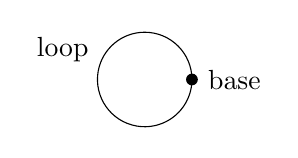
\begin{tikzpicture}
    \node[circle,fill,inner sep=1.5pt,label=right:{\dsd{base}}] (base) at (0,0) {};
    \draw (base) arc (0:170:.6cm) node[anchor=south east] {\dsd{loop}} arc (170:360:.6cm);
  \end{tikzpicture}
\end{center}
%
%
\dsd{base} is a point (object) on the circle, and \dsd{loop} is a path
(morphism) from \dsd{base} to itself.  That the circle is the free
$\infty$-groupoid on these generators means that all the points, paths,
homotopies, etc.~on the circle are constructed by applying the
$\infty$-groupoid operations to these generators in a free way.  The generator
\dsd{loop} represents ``going around the circle once
counter-clockwise.''  Using the groupoid operations, one can construct
additional paths, such as $\inv {\dsd{loop}}$ (going around the circle once
clockwise) and $\dsd{loop} \comp \dsd{loop}$ (going around the circle
twice counter-clockwise).  Moreover, there are homotopies between paths,
such as $\dsd{loop} \comp \inv {\dsd{loop}} = \dsd{id}$ (going clockwise and
then counter-clockwise is the same, up to homotopy, as staying still).
In this case, one can prove that, up to homotopy,
every loop on the circle is either \dsd{id} or $(\dsd{loop} \comp
\dsd{loop} \ldots \comp \dsd{loop})$ ($n$ times, for any $n$) or $(\inv{
\dsd{loop}} \comp \inv{  \dsd{loop}} \ldots \comp \inv{ \dsd{loop}})$ ($n$ times,
for any $n$), and thus that the loops on the circle are in bijective
correspondence with the integers.  Moreover, under this bijection, concatenation of paths corresponds to
addition of integers.  Thus, the fundamental group of the
circle is \Z.

However, in general, it can be quite difficult to relate a presentation
of a space as a free $\infty$-groupoid to an explicit description of its
homotopy groups, in part because of \emph{action across levels}.  For
example, the sphere can be presented as the free $\infty$-groupoid generated by
one point (0-cell) \dsd{base} and one homotopy (2-cell) $\dsd{loop}_2$
between $\dsd{id}_{{\dsd{base}}}$ (the path that stands still at
\dsd{base}) and itself---think of $\dsd{loop}_2$ as ``going around the
the surface of the sphere.''  An $\infty$-groupoid has group operations
at each level, so just as we have identity, inverse, and composition
operations on paths (1-cells), we have identity, inverse, and
composition operations on homotopies (2-cells).  Thus, we can form
homotopies such as $\dsd{loop_2} \comp \dsd{loop_2}$ (going around the
surface of the sphere twice) and $\dsd{loop_2} \comp \inv{\dsd{loop_2}}$
(going around the surface of the sphere once in one direction, and then
in the opposite direction)---and, analogously to above, there is a
homotopy-between-homotopies relating the latter path to the constant
homotopy ($\dsd{loop_2} \comp \inv{\dsd{loop_2}} =
\dsd{id}_{{\dsd{id}_{\dsd{base}}}}$).  Thus, one would expect that the
homotopies (2-cells) on the sphere have the same structure as the paths
(1-cells) on the circle, and this is indeed the case: $\pi_2(S^2)$ is
also \Z.  However, $\infty$-groupoids have more structure than just the
group operations at each level---for example, lower-dimensional
generators can construct higher-dimensional paths.  An example of this
is that $\pi_3(S^2)$, the group of homotopies between homotopies
(3-cells) on the sphere, is also \Z, \emph{despite the fact that there
  are no generators for 3-cells in the presentation of the sphere!}  The
paths arise from the applying the algebraic operations of an
$\infty$-groupoid to the 2-cell generator $\dsd{loop_2}$---and this
action across levels is one reason that homotopy groups are so difficult
to calculate.  

One enticing idea is to use homotopy type theory to calculate homotopy
groups: by doing so, we can give computer-checked proofs of these
calculations, and we can potentially exploit constructivity and the
type-theoretic perspective $\infty$-groupoids to attack these difficult
problems in algebraic topology.  To pose the problem of calculating a
homotopy group in homotopy type theory, we use two ingredients.  

First, we describe basic spaces using \emph{higher inductive types}, which
generalize ordinary inductive types by allowing constructors not only
for elements of the type, but for paths (proofs of equality) in the type.  For
example, the circle is represented by a higher inductive type with two
constructors
%
\[
\begin{array}{l}
\dsd{base} : S^1 \\
\dsd{loop} : \dsd{base} =_{S^1} \dsd{base} \\
\end{array}
\]
%
This says that \dsd{base} is a point on the circle, while \dsd{loop} is
a path from \dsd{base} to \dsd{base}.  In type theory, we express that 
$S^1$ is the \emph{free} type with these generators by an elimination
rule: to define a function from $S^1$ into any other type $C$, it
suffices to give a point in $c : C$, which is the image of \dsd{base}, and a
loop $p : c =_C c$, which is the image of \dsd{loop}:

\[
\begin{array}{ll}
\infer{\tptm {\Sonerec C c p} {S^1 \to C} }
      {c : C & p : c =_C c}
\end{array}
\]
That is, to define a function $S^1 \to C$, it suffices to find a
``circle'' in $C$, which gives the image of the generators.  

The computation rules for this elimination rule are as follows:
\[
\begin{array}{l}
\Sonerec C c p \dsd{base} :\equiv c \\
\dsd{ap} (\Sonerec C c p) \dsd{loop} := p 
\end{array}
\]
%
\dsd{ap} (``\textbf{a}ction on \textbf{p}aths'') applies a function $f : A \to B$ to a path $p : a =_A a'$
to produce a path $f a =_B f a'$.  Note that the first computation rule
is a definitional equality, while the second is a propositional
equality/path---while future versions of homotopy type theory might take
this to be a definitional equality, the known semantics of higher
inductive types justifies only a propositional
equality~\citep{lumsdaine+13hits}.  To express freeness, we also need to
know that $\Sonerec{C}{c}{p}$ is the unique such map, up to homotopy.  This can be
expressed either by generalizing the simple elimination rule to a
dependent elimination rule, or by adding an $\eta$-equality axiom (see
\citep{sojakova12inductive} for a discussion of these alternatives for ordinary
inductive types).  

The second ingredient is to define the homotopy groups of a type.  
One might think that we could define the homotopy groups by iterating
the identity type:

\[
\begin{array}{rcl}
\pi_1(X,x_0) & := & x_0 =_X x_0 \\
\pi_2(X,x_0) & := & \dsd{id}_{{x_0}} =_{{(x_0 =_X x_0)}} \dsd{id}_{{x_0}} \\
\pi_3(X,x_0) & := & \dsd{id}_{{\dsd{id}_{x_0}}} =_{(\dsd{id}_{{x_0}} =_{{x_0 =_X x_0}} \dsd{id}_{{x_0}})} \dsd{id}_{{\dsd{id}_{x_0}}} \\
\end{array}
\]
and so on.  However, these iterated identity types may still have
non-trivial higher-dimensional structure.  The $n^{th}$ homotopy group
considers only the structure up to level $n$, so we need to ``kill'' the
higher-dimensional structure of these types.  Thus, we first define the
\emph{$n^{th}$ loop space} $\Omega^n(X,x_0)$ so that

\[
\begin{array}{rcl}
\Omega^1(X,x_0) & := & x_0 =_X x_0 \\
\Omega^2(X,x_0) & := & \dsd{id}_{{x_0}} =_{{(x_0 =_X x_0)}} \dsd{id}_{{x_0}} \\
\Omega^3(X,x_0) & := & \dsd{id}_{{\dsd{id}_{x_0}}} =_{(\dsd{id}_{{x_0}} =_{{x_0 =_X x_0}} \dsd{id}_{{x_0}})} \dsd{id}_{{\dsd{id}_{x_0}}} \\
\end{array}
\]
and so on.  We write $\Omega(X,x_0)$ for $\Omega^1(X,x_0)$.  

Then we can define 
\[
\begin{array}{rcl}
\pi_n(X,x_0) & := & ||\Omega^n(X,x_0)||_0 \\
\end{array}
\]
where $||A||_0$, the \emph{0-truncation of $A$}, is a \emph{set} (a type
with no higher structure---any two paths are homotopic) constructed by
``killing'' the higher-dimensional structure of $A$---i.e. equating any
two paths between the same two points.  For a more leisurely
introduction to these definitions, we refer the reader to previous work~\citep{ls13pi1s1,uf13hott-book}.

Using these two ingredients, we can use homotopy type theory to
calculate homotopy groups of spaces:
define the space $X$ as a
higher inductive type, and give
a group isomorphism between the type $\pi_n(X,x_0)$ (with path
composition as the group structure) and an explicit description of a
group like $\mathbb{Z}$.  In this note, we give a calculation of the
fact that $\pi_n(S^n) = \mathbb{Z}$. That is, we describe a proof in
homotopy type theory that the $n^{th}$ homotopy group of the
$n$-dimensional sphere is isomorphic to $\mathbb{Z}$.  This proof is
interesting for several reasons:

\begin{itemize}

\item Calculating $\pi_n(S^n)$ is a fairly easy theorem in algebraic
  topology (e.g. it would be covered in a first- or second-year graduate
  algebraic topology course), but it is more complex than many of the
  results that had previously been proved in homotopy type theory.  For
  example, it was one of the first results about an infinite family of
  spaces, of variable dimension, to be proved in homotopy type theory.

\item When doing homotopy theory in a constructive/synthetic
  style in homotopy type theory, there is always the possibility that
  classical results will not be provable---the logical axioms for spaces
  might not be strong enough to prove certain classical theorems about them.
  Our proof shows that the characterization of $\pi_n(S^n)$ does follow
  from a higher-inductive description of the spheres, in the presence of
  univalence, which provides evidence for the usefulness of
  these definitions and methods.  

  Moreover, while we do not yet have a full computational interpretation
  of univalence, one can see, in the proof, a computational process that
  transforms $n$-dimensional loops on the $n$-sphere into integers.
  This is one of the first examples of computation with
  arbitrary-dimensional structures that has been considered in homotopy
  type theory.  

\item The proof is not a transcription of a textbook homotopy theoretic
  proof, but mixes classical ideas with type-theoretic ones.  
  The type-theoretic techniques used here have been applied in other
  proofs.  For example, the proof described here led to a simpler proof
  of a more general theorem, the Freudenthal Suspension Theorem
  (Lumsdaine's proof is described in the HoTT book~\citep{uf13hott-book}), which
  gives a shorter calculation of $\pi_n(S^n)$ (also described in the
  HoTT book).  This, in turn, led to a proof of an even more general
  theorem, the Blakers-Massey theorem~\citep{fll13blakersmassey}.  

\item We give a direct higher-inductive definition of the
  $n$-dimensional sphere $S^n$ as the free type with a base point
  \dsd{base} and a loop in $\Omega^n(S^n)$.  This definition does not
  fall into the collection of higher inductive types that has been
  formally justified by a semantics, because it involves a path
  constructor at a variable level (i.e. in $\Omega^n$, where $n$ is an
  internal natural number variable).  However, our result shows that it is a useful
  characterization of the spheres to work with, and it has prompted some
  work on generalizing schemas for higher inductive types to account for
  these sorts of definitions.

\item The proof we present here includes an investigation of some of the
  type-theoretic structure of loop spaces.  We will characterize
  $\Omega^n(A)$ for various types $A$, which explains how concepts such
  as function extensionality and univalence induce paths at higher
  levels.  This characterization could potentially inform investigations
  into the computational interpretation of univalence, a major open
  problem.  

\item The proof has been formalized in Agda~\citep{norell07thesis}, and
  is available on GitHub in the repository
  \url{github.com/dlicata335/hott-agda} (tag \ttt{pinsn-cpp-paper}).  The proof includes a library
  of lemmas about iterated loop spaces that is independent of the
  particular application to $n$-dimensional spheres.
\end{itemize}

In the remainder of this paper, we give an informal overview of some
of the interesting aspects of the proof, and discuss the Agda
formalization.  From this point forward, we assume that the reader is
familiar with the calculation of $\pi_1(S^1)$~\citep{ls13pi1s1} and with
Part I and Chapter 8 of the HoTT book~\citep{uf13hott-book}.  

%%% Local Variables:
%%% mode: latex
%%% TeX-master: "paper"
%%% End:
